\documentclass{article}

\usepackage[english]{babel}

\usepackage[letterpaper,top=2cm,bottom=2cm,left=3cm,right=3cm,marginparwidth=1.75cm]{geometry}

% Useful packages
\usepackage{amsmath}
\usepackage{graphicx}
\usepackage[table,xcdraw]{xcolor}
\usepackage[colorlinks=true, allcolors=blue]{hyperref}

\begin{document}

\title{Universal NAND and NOR}
\author{Ella Xu, Digital Electronics}
\maketitle

\section{Alarm}

\subsection{AOI}

\begin{figure}[!htb]
\centering
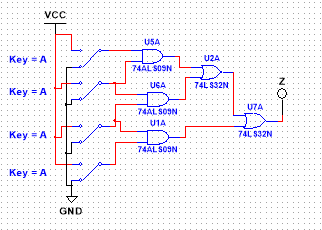
\includegraphics[width=0.6\textwidth]{images/AlarmAOI.PNG}
\caption{\label{fig:alarm aoi}This is the AOI logic circuit of the Alarm.}
\end{figure}

\subsection{Universal NOR}

\begin{figure}[!htb]
\centering
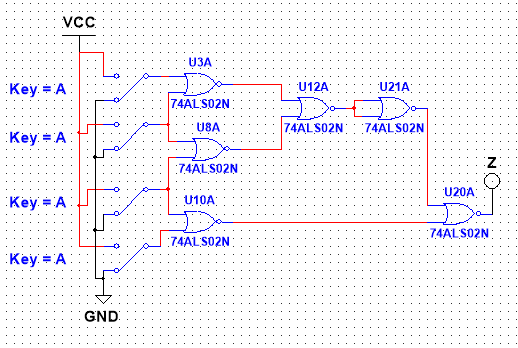
\includegraphics[width=0.6\textwidth]{images/AlarmUniversalNOR.PNG}
\caption{\label{fig:alarm nor}This is the logic circuit for the Alarm using universal NOR gates.}
\end{figure}

\subsection{Universal NAND}

\begin{figure}[!htb]
\centering
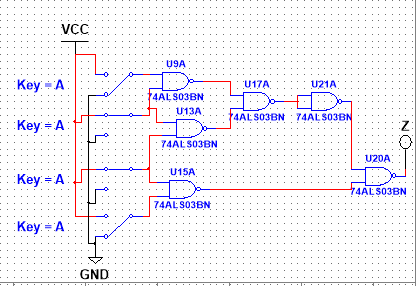
\includegraphics[width=0.6\textwidth]{images/AlarmUniversalNAND.PNG}
\caption{\label{fig:alarm nand}This is the logic circuit for the Alarm using universal NAND gates.}
\end{figure}

\section{Booth}

\subsection{AOI}

\begin{figure}[!htb]
\centering
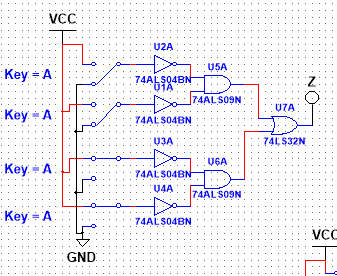
\includegraphics[width=0.6\textwidth]{images/BoothAOI.PNG}
\caption{\label{fig:booth aoi}This is the AOI logic circuit of the Booth.}
\end{figure}

\newpage

\subsection{Universal NOR}

\begin{figure}[!htb]
\centering
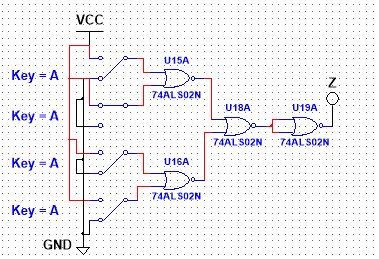
\includegraphics[width=0.6\textwidth]{images/BoothUniversalNOR.PNG}
\caption{\label{fig:booth nor}This is the logic circuit for the Booth using universal NOR gates.}
\end{figure}

\subsection{Universal NAND}

\begin{figure}[!htb]
\centering
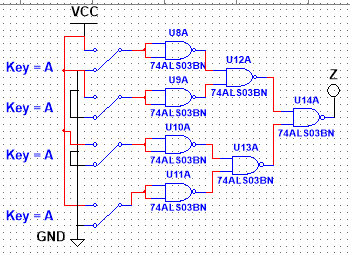
\includegraphics[width=0.6\textwidth]{images/BoothUniversalNAND.PNG}
\caption{\label{fig:booth nand}This is the logic circuit for the Booth using universal NAND gates.}
\end{figure}

\end{document}